%===================================== CHAP 2 =================================
\cleardoublepage

\chapter{Theory}
The main research goal and RQ1 is to give recommendations by utilizing CBR, therefore it is essential to understand how CBR works. This chapter presents a brief introduction to the CBR methodology and Case-Based Recommender Systems, explains MyCBR; the tool which will be used to implement the CBR part of the system, and presents theory on motivation relevant to RQ2.


\section{Case-based Reasoning}
Case-Based Reasoning (CBR) is a methodology in AI for solving problems, and is essentially based on experience. This experience can be used to solve a large range of problems, including complex combinatorial problems, or yield solutions where uncertainty is involved\cite{richter2013case}. Implied by the name, CBR can be broken down into two main concepts; \textit{cases} and \textit{reasoning}.

\begin{enumerate}
    \item \textbf{Case:} An experience of a solved problem, usually represented as a feature vector (see section \ref{sec:feature_vectors}). A case consists of two parts: a problem description and a solution to the problem. A Case-Based Reasoning System stores all of its cases in a \textit{Case Base}.
    \item \textbf{Reasoning:} The approach of drawing conclusions using cases, given a problem to be solved.
\end{enumerate}

Reasoning in CBR differs from other kinds of reasoning because it does not lead from true assumptions to true conclusions. This means that for two cases with identical problem descriptions, the solution to one of them might not be the solution for the other. The recorded experience in the first case may not be exactly similar to the other case. To be reused, it only has to be \enquote{similar}.

\subsection{Feature Vectors}\label{sec:feature_vectors}
A case is usually represented as a feature vector, consisting of a few to many pairs of attributes and their values. A common example is the diagnosis of a sick patient, where a collection of symptoms and weather the patient has them is the problem description, and the final diagnoses is the solution to the case, as illustrated by Table \ref{tab:example_case}

\begin{table}[H]
\centering
\small
\caption{A classic case representation with attribute-value pairs for the problem description and the solution.}
\label{tab:example_case}
\begin{tabulary}{\textwidth}{|L|L|}
\hline

\textbf{Attribute}           & \textbf{Value}     \\ \hline
Nausea              & Yes       \\ \hline
Fever               & Yes       \\ \hline
Malaise             & Dizzy     \\ \hline
Blood pressure      & Normal    \\ \hline
Vision changes      & No        \\ \hline
Shortness of breath & No        \\ \hline
Diagnosis           & Influenza \\ \hline
\end{tabulary}
\end{table}

\subsection{The CBR-Cycle}\label{sec:cbr-cycle}

Aamodt \& Plaza\cite{aamodt1994case} defined a model which explain the problem solving cycle in CBR, see figure \ref{fig:cbr_cycle}. The cycle defines four distinct processes which a case goes through, which can be summarized as follows.

\begin{description}
\item [Retrieve:] The most similar case is retrieved from the system's case base, so that it can be compared to a new case.
\item [Reuse:] The solution to the retrieved case is applied to the new case.
\item [Revise:] Confirms that the proposed solution solves the new case, or if its not applicable.
\item [Retain:] Retains the new case with the given solution in the case base for future usage.
\end{description}

\begin{figure}[H]
    \centering
    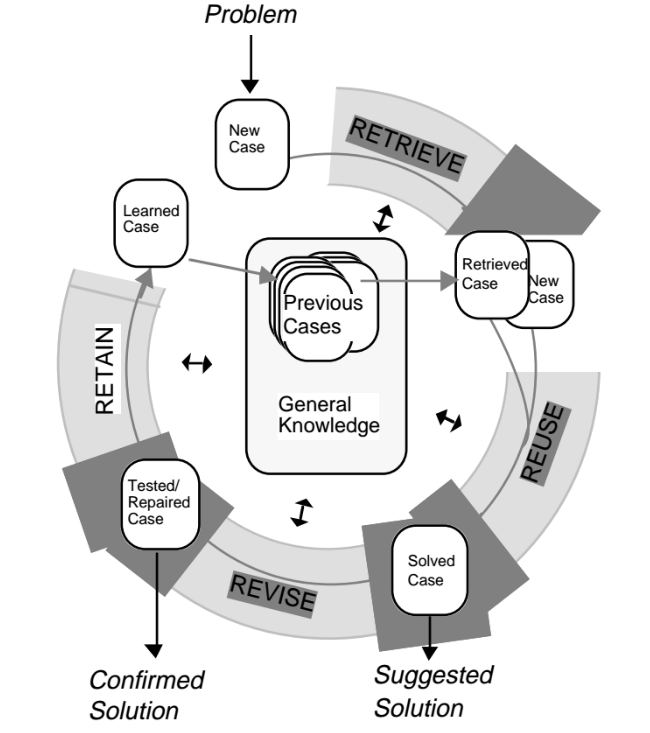
\includegraphics[width=0.6\textwidth]{fig/cbr_cycle.png}
    \caption{The CBR Cycle}
    \label{fig:cbr_cycle}
\end{figure}

\subsection{Similarity Measures}
The degree of similarity between a set of input variables, and a case stored in the case-base is calculated and represented as a \emph{Similarity Measure} (SM). Naturally, a CBR system returns the case or cases where the SMs yielded the highest similarity score. How the similarity score is calculated is different for each configuration, and must be tailored to each specific system. Typically, each attribute in a case has its own function for calculating the similarity to the appropriate input-attribute. The most suitable function depends on the attribute's type. For example will a typical function for an integer or float be the distance from the input value, at a given step, while for a string symbol, it can be the result of approximate string matching. Each attribute is given a weight, which decides which attributes are most important, and finally the similarity for each attribute is joined with a sum function, with their weights in consideration.

\subsection{Case-based Reasoning Systems}
A Case-based Reasoning System is a system which use the CBR methodology to solve problems. When it receives a new problem, it first performs step 1 in the CBR-cycle (retrieve). It then selects the case in its case-base which is the most similar to the new problem by using the designated similarity measure on each attribute in the case with regards to the similar attribute in the problem. When the most similar case has been selected, that case's solution is applied to the new problem (step 2, reuse). The proposed solution to the new problem is revised, tested and or repaired (step 3), before new problem with its new solution is retained as a new case in its case base.

\section{MyCBR}

MyCBR is a tool for rapid prototyping of CBR systems with focus on the retrieval step of the CBR cycle.\cite{MyCBR}. Its developed and maintained as a joint project between the German Research Center for Artificial Intelligence (DFKI) and the School of Technology and Computing at the University of West London (UWL)\cite{Stahl2008}. MyCBR was chosen as the designated tool to model the CBRS, because it includes all the necessary functionality, as well as requireing a minimum of domain knowledge, and knowledge about the tool itself. Furthermore, using this tool would make getting help and support easier, considering NTNU has an employee whom is a contributor to the project. MyCBR was used extensively throughout the project to assist with both prototyping and modelling the CBRS. The MyCBR project is first and foremost a Java Software Development Kit (SDK), but also includes a pre-built GUI called the MyCBR Workbench. 

\subsection{MyCBR SDK}
The MyCBR SDK provides an access point for implementing the functionality of MyCBR in a custom application. The SDK is written in the JAVA programming language and has executable programs for macOS, Windows and Linux\cite{MyCBR}. 

The current version of the SDK and MyCBR focuses and has implemented only the similarity based retrieval step of the CBR cycle. The myCBR developers reason that this it is due to most applications having the first part as its core functionality\cite{Stahl2008}.  

A recent update extended the SDK to include a REST API that enables cross server communication and requests to MyCBR. This allows an external server to use many of the implemented functionalities in MyCBR SDK as Querying and retrieval.

\subsection{MyCBR Workbench}

The myCBR workbench provides a graphical user interface (GUI) of the features in the SDK. This allows easier prototyping and usage for users without the need to have large knowledge of the SDK's inner functions\cite{bach2014knowledge}. 

To be able to quickly import data and cases, the workbench supports importing pre-defined cases with the CSV file format. All the required cases can therefore be gathered and refined before being tested in the workbench. The workbench also supports a set of similarity functions that are easy to model such as Taxonomy and integer functions. The workbench visualises these similarity measures with graphs and tables.

\begin{figure}[H]
    \centering
    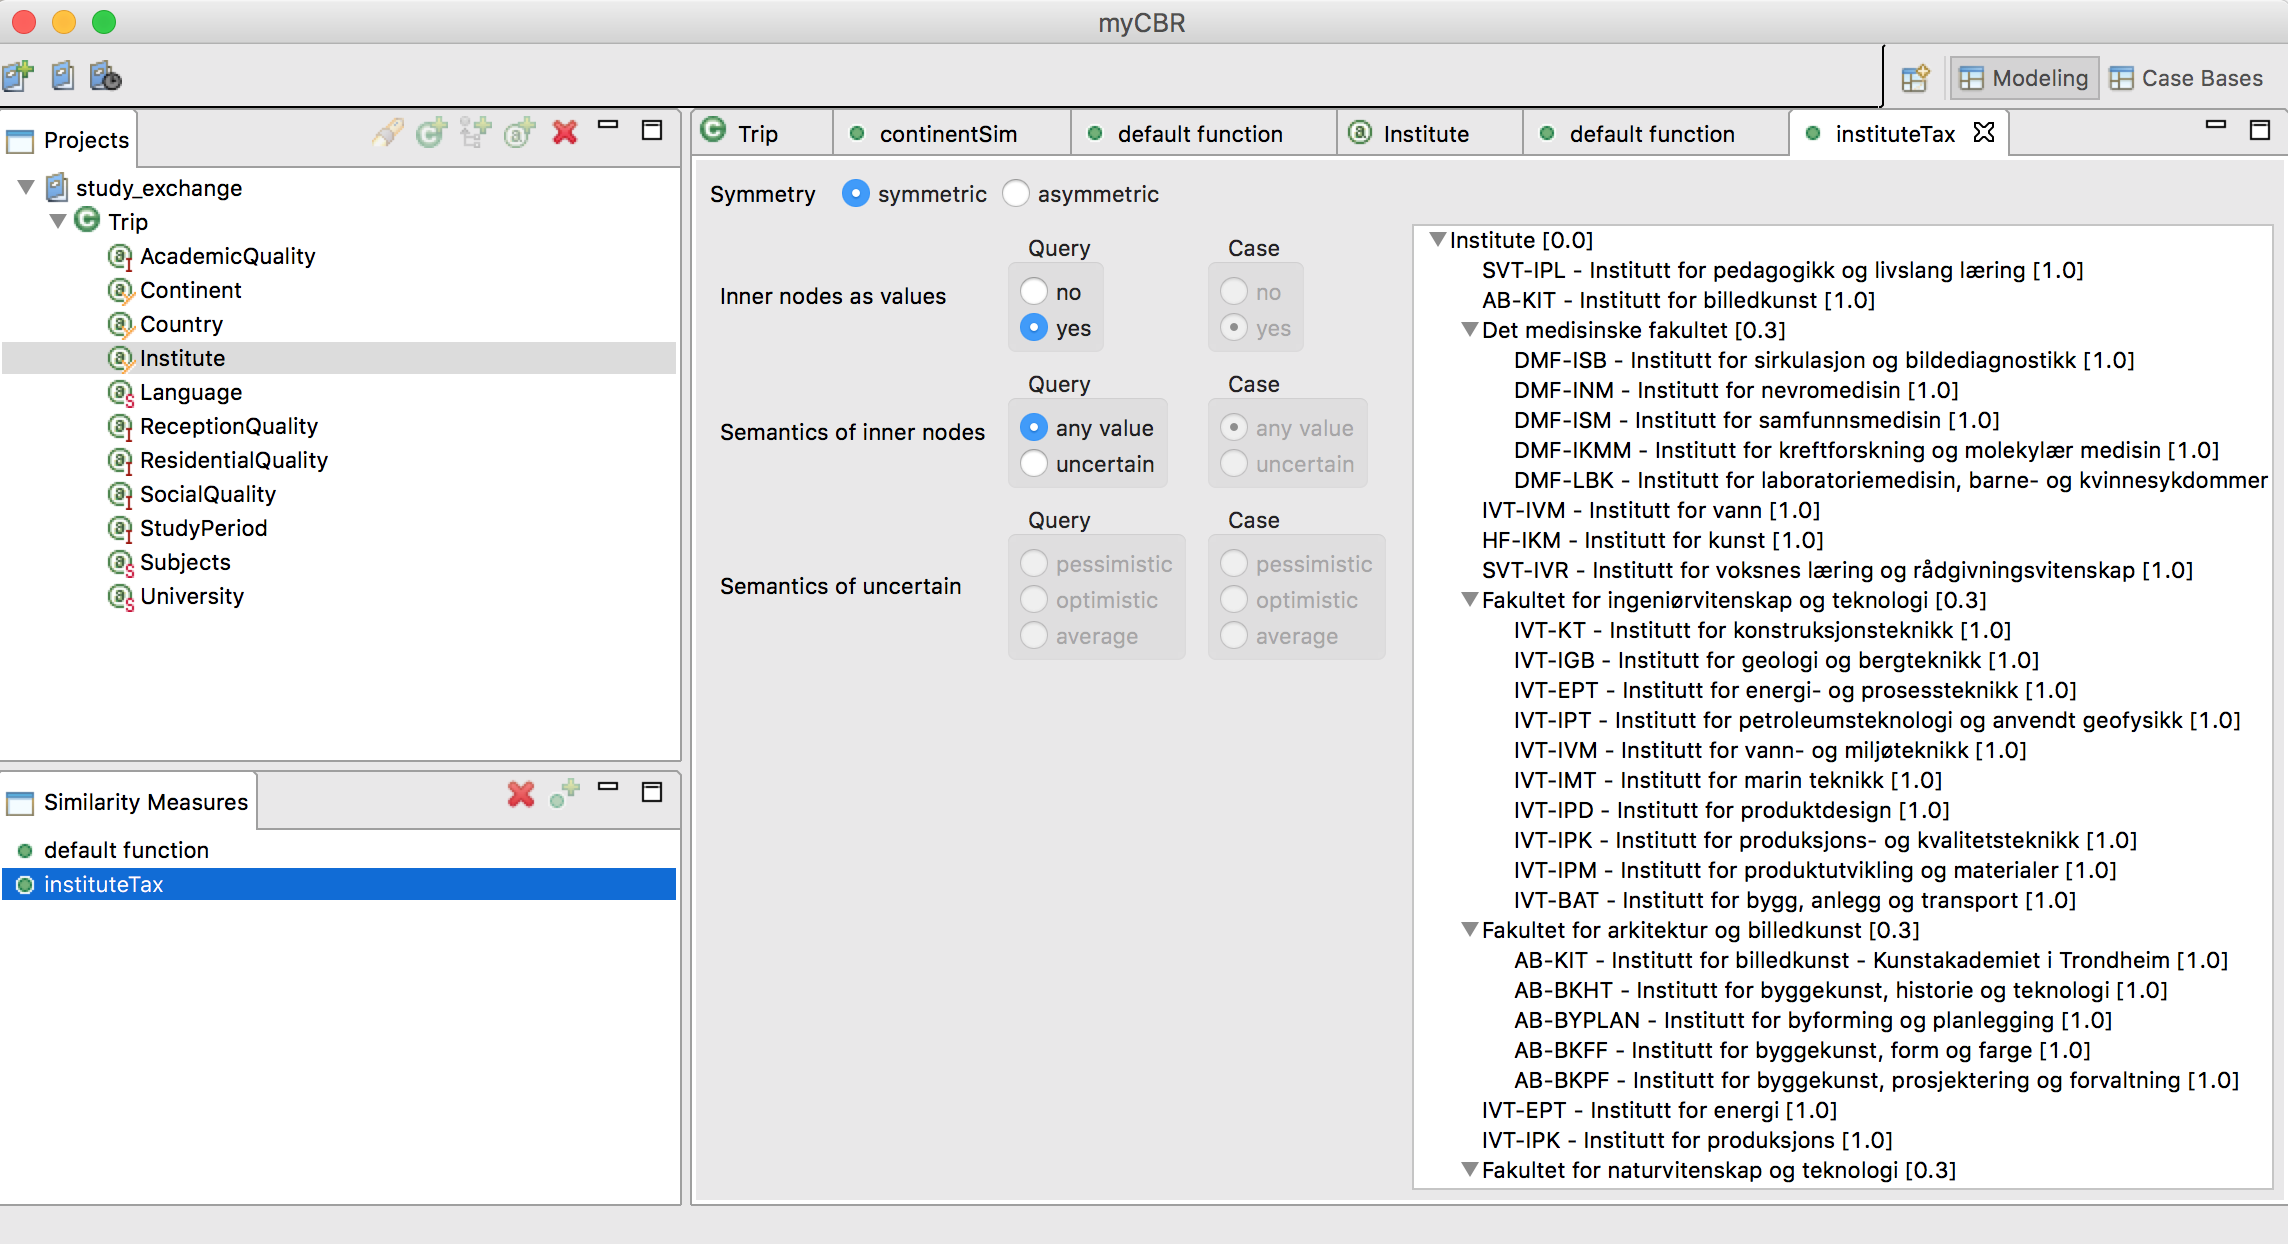
\includegraphics[width=8cm]{fig/myCBRworkbench.png}
    \caption{Example of modelling the taxonomy function from myCBR workbench}
\end{figure}

\subsection{Similar tools}
Due to the increasing popularity of CBR applications\cite{kolodner2014case}, many tools have been developed to model and implement a CBRS. These tools makes it easier to quickly develop CBRS prototypes without having to start from scratch. This section will introduce some of the different approaches to tool-kits and the reasoning for the selected tool of this research project. 

\paragraph{JColibri}
is an object-oriented framework in Java for building CBR systems, which follows the task/method division paradigm.\cite{bello2004jcolibri} The notion of this paradigm is that each task in a CBR-cycle described in section \ref{sec:cbr-cycle} involves several specific sub-tasks, and instead of using one method on each task, they are decomposed and structured in a way so that different methods can be applied to the different sub-tasks. All though this framework is flexible in terms of the problem domain it will be used for, and can be used for any number of the steps in the CBR-cycle, it required a substantial amount of knowledge for the developers because they have to use appropriate methods for different tasks, go more in depth than other frameworks.

\paragraph{FreeCBR}
is a freeware CBR-system which both offers a graphical user-interface as well as a command line. All though beeing a quite simple system, it is still capable of handling a large range of problem domains, by determining the similarity of attributes of regular types such as Float, Integer, Bool and String. This tool was for example used in a project where it determined the best plays in a poker game \cite{sandven2006case}. All though the system in this research, similar to a game of poker, attempts to recommend the course of action where uncertainty is present, the MyCBR offers a larger range of attribute types and similarity measures, which was assumed to be necessary in this project.


\section{Case-based Recommender Systems}\label{sec:case_based_recommender_systems}
Recommendation systems mainly use two different approaches, either collaborative or case-based. The collaborative approach uses the rating and opinions of other users who have experienced the product or gone through the same process. The case-based approach used a case base as the pool of information to pick recommendations from.

Case-based recommender systems (CBRS) share many similarities with case-based reasoning systems, most noteworthy that both type of systems have a case base which they use to determine the best solution, recommendation or course of action. The queries a CBRS receive are often structured more like a wish.\cite{richter2013case} This wish includes preferences the users set themselves, and profile information. The main difference lies in the way the systems propose a solution to a problem; instead of proposing the case which matches a problem the best, a CBRS typically propose multiple suggestions which should be relevant for the user. Similar to a case-based reasoning system, a CBRS use CBR as the underlying methodology. However, for a CBRS the adaption part of the CBR cycle is not always that important; the most essential part is step 1, retrieval. The main focus of the system is to recommend something, not to directly solve a problem. 

The use of similarity-based retrieval is a beneficial feature of case-based recommenders, giving advantages over more traditional exact matching techniques such as conventional database retrieval and classical constraint satisfaction techniques\cite{bridge2005case}.

Recommender systems are used extensively in both research and commercial products. These systems provide several possible solutions that might be viable for the user to choose. Several published research papers have explored different approaches to recommender systems\cite{mulyana2015case}\cite{quijano2011happy}. 

\subsection{Evaluating recommender systems}
Guy Shani \& Asela Gunawardana (2011)\cite{shani2011evaluating} reviews three processes of evauluating recommendation systems; offline experiments, online evaluation, and user studies.

Recommendation systems are often evaluated and ranked based on their prediction power\cite{shani2011evaluating}. Because recommendation often is a subjective manner, it is however hard to simply evaluate this. Some users would like to find something new, in which they don't currently know if is a good suggestion or not, while some users want to see a more diverse pool of suggestion than others\cite{shani2011evaluating}. To evaluate these systems, researchers can either define what good recommendations are, and perform offline experiments with simulated user queries, ask and observe users of the system and see if they think the recommendations are good, or implement algorithms which evaluate the system as it is used online.

\section{Motivation}
Richard M. Ryan and Edward L. Deci (2000)\cite{ryan2000intrinsic} divides motivation into two categories; Intrinsic- and Extrinsic motivation. Intrinsic motivation defines inner motivation such as doing something simply for enjoyment, satisfaction or out of interest. Extrinsic motivation is a much broader category which pertains whenever an activity is done in order to attain some separable outcome\cite{ryan2000intrinsic}. For example, a student might be motivated perform well on a test because they want to receive a good grade, and not because they enjoy the theory at hand. Carol M. Sánchez et al. (2006)\cite{sanchez2006motivations} finds that most of the intent of a group of U.S., French, and Chinese Students stems from intrinsic motivation- doing it for their own enjoyment. 

What about students who are interested and motivated to go on exchange, but end up not doing it? Mazzarol and Soutar (2002)\cite{mazzarol2002push} finds that students' general motivation is influenced by the amount of information available at a university and its courses, and that \enquote{knowledge and awareness} proved to be the most influencing factor when choosing an international study location. Even though a student may have the intrinsic motivation to go on an exchange, the process of applying for an exchange itself may be non-intuitive, cumbersome, or the related information might be difficult to find. 



\cleardoublepage